% CREATED BY DAVID FRISK, 2016
\chapter{Background}
\section{Introduction to reinforcement learning}
\subsection{Problem setting}
In the usual engineering approach to problems,
prior scientific knowledge is used to first describe the problem
and then to define it mathematically.
Once this is done, unknown variables are measured and
solutions are calculated.
This approach works if the inherent stochasticity of the environment
can be controlled, i.e. if bounds of stochasticity are known
the solution account for them and be designed to be robust to them.
But some problems have circumstances which can not be known in advance,
or which are incredibly hard to hand-engineer.

In those cases, an entirely different approach becomes the only viable one:
designing a system which can produce and refine its own solution,
or in other words, designing a system which, in a way, learn the
solution by itself.
This is the idea behind the learning-based approach: automating the 
process of learning.
Crucially, now the world and how it operates
is unknown and has to be discovered.  
The schematic \ref{fig:rl-shematic} shows how this process is formulated in reinforcement learning.
\begin{figure}[htpb]
\begin{center}
\begin{tikzpicture}[scale=1, transform shape, node distance=2.0cm]
		\node (agent) [rec] {agent};
		\node (environment) [rec, right of=agent, xshift=1.5cm] {environment};
		\draw [arrow, xshift=0.5cm]  (environment.240) to [bend left=30] node [midway, below, yshift=-0.2cm] (textnode1) {observation, reward}  (agent.300);
		\draw [arrow, xshift=0.5cm]  (agent.70) to [bend left=30] node [midway, above, yshift=0.2cm] (textnode2) {action} (environment.100);
\end{tikzpicture}
\end{center}
\caption{Conceptual schematic of reinforcement learning.}
\label{fig:rl-shematic}
\end{figure}
Reinforcement learning is a 2-step iterative process.
The \textbf{agent}, which represents the computer program, takes \textbf{actions}
in its \textbf{environment}. It then \textbf{observes} the resulting state
of the environment and is also given a \textbf{reward}
which is a function mapping every state of the environment to a number.

To introduce reinforcement learning more formally,
we first describe the simplest possible problem 
to which reinforcement learning is the best solution.

\subsection{Bandit problems}
Reinforcement learning  uses training information that evaluates 
the actions taken rather than instruct by giving correct actions.
Consider this learning problem.
The agent is faced with $k$ different gambling slot machines.
Each of them give random rewards under an unknown distribution.
At each turn, the agents has to select one of the machines and pull its lever.
%The agents is repeatedly faced with a choice of k different actions.
%After each choice the agent receive a numerical reward based on the action selected.
The goal is to maximize the expected total reward over some number of turns.
%This is original form of k-armed bandit problem.
%Depending on the action selected $k$-armed bandit problem formalizes the value function to get the expected or average reward.
If the agent knew the distribution of rewards of each of the slot machines, 
it would simply choose the one with the highest expected reward in number of turns 
it has been given.
%It is assumed the agent do not know the action value with certainty although the estimate of 
%the action value is known by the agent and we expected it to be close to actual value of the action.
At any time step the agent will be able to select at least one action whose estimated value is greatest.
When the agent selects on of this actions it is exploiting the current knowledge of the
values of the actions.
If the agents keep exploiting the goal of maximizing reward over period of time will be trivial.
If instead the agent selects one of the non greedy action this will enables it to improve the average expected reward over time.
 
When addressing the canonical problem of sequential decision making under uncertainty,
the exploitation-exploration trade-off is highlighted.More specifically,
as depicted in Fig.1, an agent interacts with an unknown environment in a sequential manner to obtain rewards.
The ultimate goal is to maximize the rewards.
For one thing, the agent takes advantage of existing knowledge of the environment.
For another, the agent investigates an unfamiliar environment.
%Reinforcement Learning, which includes Multi-Armed Bandit (MAB), Markov Decision Process (MDP), and Partially observable Markov Decision Process, is always used to formalize the exploit-exploration trade-off (POMDP).

%\begin{figure}[H]
%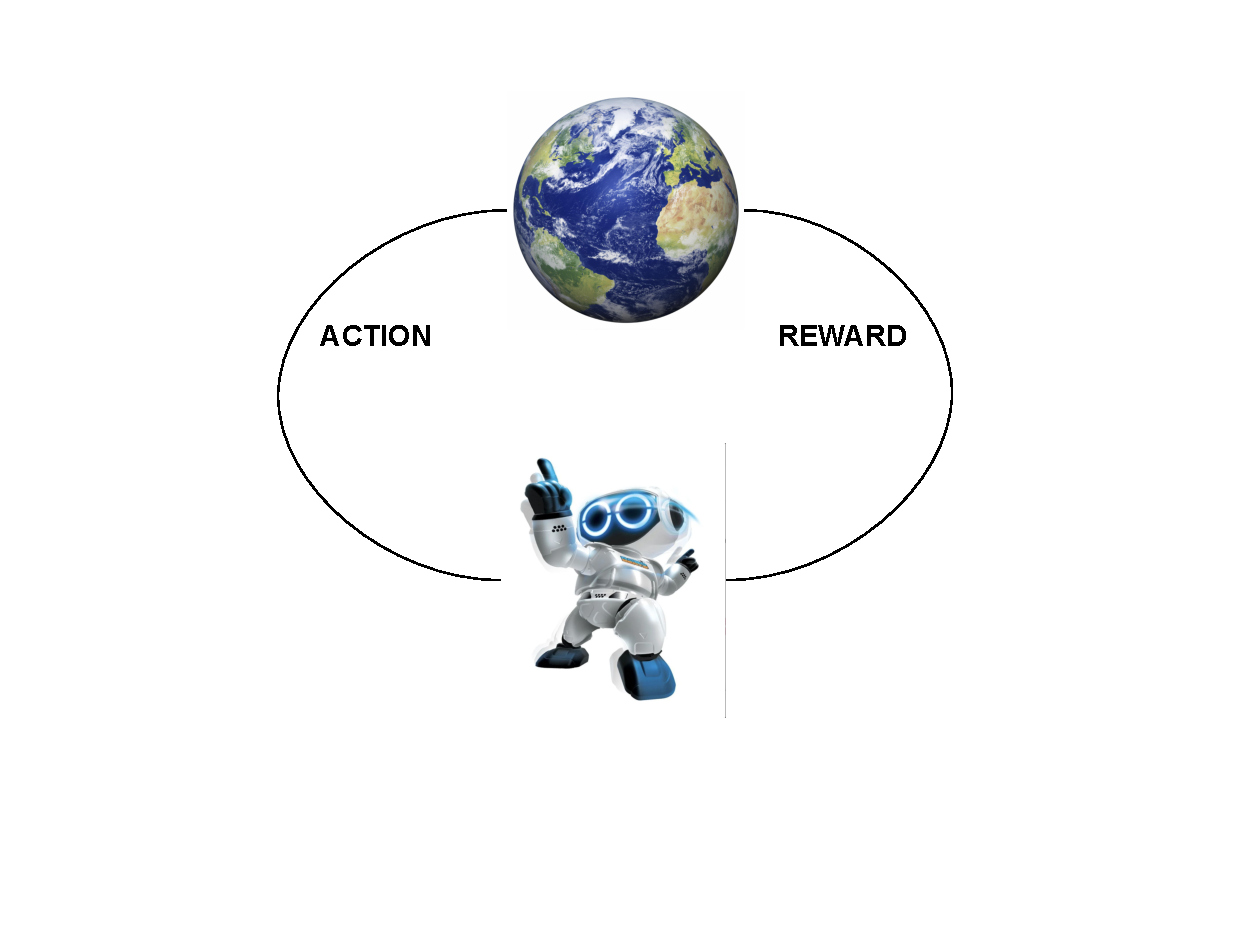
\includegraphics[width=12cm]{figure/RL_representation.pdf}
%\caption{An agent sequentially interaction with unknown environment and receive the rewards }
%\centering
%\end{figure}

%According to many studies of Reinforcement Learning,the unknown environment can described by multiple elements  including observations $\Omega$, states S, actions A, reward function R, state transition probability T, and conditional observation probabilities O.Bandit, MDP, and POMDP models the environment by considering different elements respectively.The formalisation of reward and policy in each model is different kinds of which leads to multiple techniques to learn.In the table 1  the relationship among bandit, MDP, RL, and decision theory are presented.In the next section we discuss the formalisation of MDPs for modern reinforcement learning.


\begin{table}[H]
\caption{Li Zhou ,relationship among bandit, MDP, RL, and decision theory}
\begin{tabular} {l|l|l}\hline\hline
$Learn model out come$  &  Mutlti armed bandits  &   RL \\ \hline
$Given model of stocastic out comes $ &  Decision Theory & MDP  \\ \hline\hline
$    $ &  Actions dont  
change state of the world & Actions change 
state of the world  \\ \hline\hline
\end{tabular}
\end{table}

%\textbf{TODO ADD EQUATION:
%   -FIT THE TABLE
%   -copy past the related work from the other notes
%   -rewrite some of the algorithms}
 
\subsection{Markov Decision Processes}
%\cite{gehring2017convolutional}
The environment of $ k  $-bandit problem is static --- 
the actions do not change the \textbf{state} of the environment.
To model environments in which states change, Markov chains are used.
They capture the stochastic nature of state transitions, while Markov property 
allows for easier mathematical analysis.
The schematic of a Markov chain is shown in \ref{fig:markov-chain}.

\begin{figure}[htpb]
\begin{center}
\begin{tikzpicture}[scale=1, transform shape, node distance=1.5cm]
		\node (s1) [mcs] {$\bm{s}_{1} $};
		\node (s2) [mcs, right of=s1, xshift=1cm] { $ \bm{s}_{2}  $};
		\draw [arrow] (s1) -- node [below, midway] {$ p(\bm{s}_{t+1}|\bm{s}_{t}) $} (s2);
		\node (s3) [mcs, right of=s2, xshift=1cm] { $ \bm{s}_{3}  $};
		\draw [arrow] (s2) -- node [below, midway] {$ p(\bm{s}_{t+1}|\bm{s}_{t}) $} (s3);
\end{tikzpicture}
\end{center}
\caption{Schematic of a Markov chain.}
\label{fig:markov-chain}
\end{figure}

Formally, a Markov chain $ \mathcal{M}  $is the defined by its state space
$ \mathcal{S}  $ with discrete or continous state $ \bm{s} \in \mathcal{S}  $
and the transition operator $ \mathcal{T}  $.
The notation $ \bm{s}_{ t }  $ denotes the state at time $ t  $ and it is a vector of real numbers.
The transition operator allow for a succinct description of environment dynamics.
For a transition probability $ p(s_{ t+1 }|s_{ t })  $,
let $ \mu_{ t,i } = p (\bm{s}_{t} = i)  $ and
$ \mathcal{T}_{ i,j } = p (\bm{s}_{t+1} = i|\bm{s}_{t} = j )  $.
Then $\overrightarrow{\mu}_t$ is a vector of probabilities and 
$\overrightarrow{\mu}_{t+1} = \mathcal{T} \overrightarrow{\mu}_t$.
Importantly, $ \mathcal{T}  $ is linear.

To model the agent's actions, we simply augment the Markov chain by adding
actions as priors to state transition probabilities and defining the reward function, 
thereby constructing a Markov decision process.
It's schematic can be seen in \ref{fig:mdp}.
\begin{figure}[htpb]
\begin{center}
\begin{tikzpicture}[scale=1, transform shape, node distance=1.5cm]
		\node (s1) [mcs] {$\bm{s}_{1} $};
		\node (a1) [mcs, above right of=s1] { $ \bm{a}_{1}  $};
		\node (s2) [mcs, right of=s1, xshift=1.5cm] { $ \bm{s}_{2}  $};
		\draw [arrow] (a1) -- (s2);
		\draw [arrow] (s1) -- node [below, midway] {$ p(\bm{s}_{t+1}|\bm{s}_{t}, \bm{a}_{t}) $} (s2);
		\node (s3) [mcs, right of=s2, xshift=1.5cm] { $ \bm{s}_{3}  $};
		\node (a2) [mcs, above right of=s2] { $ \bm{a}_{2}  $};
		\draw [arrow] (s2) -- node [below, midway] {$ p(\bm{s}_{t+1}|\bm{s}_{t}, \bm{a}_{t}) $} (s3);
		\draw [arrow] (a2) -- (s3);
\end{tikzpicture}
\end{center}
\caption{Schematic of a Markov decision process.}
\label{fig:markov-chain}
\end{figure}

The Markov decision process is thus defined by the tuple
$ \mathcal{M} = \{\mathcal{S}, \mathcal{A}, \mathcal{T}, r\}  $.
$ \mathcal{A}  $ denotes the action space, where
$ \bm{a}_{} \in \mathcal{A}  $ is a continous or discrete action and
$ r  $ is the reward function $r : \mathcal{S} \times \mathcal{A} \to \mathbb{R}$.
It should also be noted that now the transition operator is a tensor.
Let $\mu_{t,j} = p(s_t = j), \xi_{t,k} = p(a_t = k), \mathcal{T}_{i,j,k} = p(s_{t+1} = i | s_t =j, a_t =k) $.
Then $\mu_{t+1,i} = \sum_{j,k}^{} \mathcal{T}_{i,j,k} \mu_{t,j} \xi_{t,k}$.
Hence $ \mathcal{T}  $ retains its linearity.

Finally, partial observability also needs to be accounted for.
To do so, a partially observable Markov decision process (POMDP) needs to be constructed.
This is done by augmenting the Markov decision process to also include
the observation space $ \mathcal{O}  $, where observations $ \bm{o}_{} \in \mathcal{O} $
denote the discrete or continous observations
and the emission probability $ \mathcal{E}  $ which describes the probability 
$ p(\bm{o}_{t} | \bm{s}_{t})  $ of getting the observation $ \bm{o}_{t}  $ when in state  $\bm{s}_{t}$.
The schematic can be seen in \ref{fig:pomdp}.

\begin{figure}[htpb]
\begin{center}
\begin{tikzpicture}[scale=1, transform shape, node distance=1.5cm]
		\node (s1) [mcs] {$\bm{s}_{1} $};
		\node (a1) [mcs, above right of=s1] { $ \bm{a}_{1}  $};
		\node (o1) [mcs, above of=s1] { $ \bm{o}_{1}  $};
		\draw [arrow] (s1) -- (o1);
		\node (s2) [mcs, right of=s1, xshift=1.5cm] { $ \bm{s}_{2}  $};
		\node (o2) [mcs, above of=s2] { $ \bm{o}_{2}  $};
		\draw [arrow] (s2) -- (o2);
		\draw [arrow] (a1) -- (s2);
		\draw [arrow] (s1) --  (s2);
		\node (s3) [mcs, right of=s2, xshift=1.5cm] { $ \bm{s}_{3}  $};
		\node (o3) [mcs, above of=s3] { $ \bm{o}_{3}  $};
		\draw [arrow] (s3) -- (o3);
		\node (a2) [mcs, above right of=s2] { $ \bm{a}_{2}  $};
		\draw [arrow] (s2) -- (s3);
		\draw [arrow] (a2) -- (s3);
\end{tikzpicture}
\end{center}
\caption{Schematic of a partially observable Markov decision process.}
\label{fig:pomdp}
\end{figure}
It is important to note that not all elements of POMDP are present in every problem: for example,
the reward may be a determinstic function of the state and so on.
In general through the text, to aid in simplifying notation, only the necessary elements will be explicity referenced
in sketches and written out in the equations (most often using just the Markov decision process).
%However, POMDP fully describes the setting in which reinforcement learning algorithms can be defined.


%Markov decision processes (MDPs) are used to model decision making in discrete, stochastic, sequential environments,
%and are thus a natural choice of model in which reinforcement learning can be defined.
%[9].
%Markov Chain, which works with S, a set of states, and P, the probability of transitioning from one to the next. It also uses the Markov Property, meaning each state depends only on the one immediately prior to it.

%MDPs is a framework that can solve most of reinforcement learning problems with discrete actions.The formal definition of Markov decision process can be summarised in  the tuple $\mathcal{M} = \{\mathcal{S}, \mathcal{A},\mathcal{P(S_0)}, \mathcal{T}, r\}$[8].
%The goal of the model is that an agent inhabits a  stochastic environment in a response to action choice made by the agent[9]. \\

%The environment consists of the the Transition function, $\mathcal{T} : \mathcal{S} \times \mathcal{A} \to \mathcal{(PS)}$.\\  and the reward function ($r(s_t, a_t)$), $r : \mathcal{S} \times \mathcal{A} \to \mathbb{R}$.In MDPs the transition probability and reward only depends on the current state and the action chosen by the agent  but not the past state and action.

%The agent acts in environment according to a policy $\mathcal{\pi} : \mathcal{S} \to \mathcal{(PS)}$.policy learned can be off policy where the behaviour policy is different from the policy used for action selection one common example is Q-learning or on-policy methods which attempts to evaluate or improve the policy that is used to make decision.\\
%The former state-action value function (Q function for short)can be computes recursively with dynamic programming: 


\subsection{Key concepts in reinforcement learning}
\subsubsection{Policy}
With the problem space being formally defined,
we may introduce definitions which will allow the construction
of reinforcement learning algorithm.
The reinforcement learning problem can be defined in finite or infinite time horizons.
Different environments usually naturally fall in either category.
For the agent to learn, it needs to be able to try out different actions from the same, 
or at least similar states.
This is usually achieved by having the agent return to a set of starting states.
The period between two such returns is called \textbf{an episode}.
The agent selects actions based on its \textbf{policy} $ \pi  $.
The policy is a function which maps states to actions.
The schematic showing it in the context of a Markov decision process
is given in \ref{fig:policy-in-mdp}.
\begin{figure}[htpb]
\begin{center}
\begin{tikzpicture}[scale=1, transform shape, node distance=2.5cm]
		\node (s1) [mcs] {$\bm{s}_{1} $};
		\node (a1) [mcs, above right of=s1] { $ \bm{a}_{1}  $};
		\node (s2) [mcs, right of=s1, xshift=1.5cm] { $ \bm{s}_{2}  $};
		\draw [arrow] (a1) -- (s2);
		\draw [arrow] (s1) -- node [below, midway] {$ p(\bm{s}_{t+1}|\bm{s}_{t}, \bm{a}_{t}) $} (s2);
		\node (s3) [mcs, right of=s2, xshift=1.5cm] { $ \bm{s}_{3}  $};
		\node (a2) [mcs, above right of=s2] { $ \bm{a}_{2}  $};
		\draw [arrow] (s2) -- node [below, midway] {$ p(\bm{s}_{t+1}|\bm{s}_{t}, \bm{a}_{t}) $} (s3);
		\draw [arrow] (a2) -- (s3);
		\draw [arrow] (s1) -- node [above, midway, sloped] {$\pi_{ \theta } (\bm{a}_{t}| \bm{s}_{t} )  $} (a1);
		\draw [arrow] (s2) -- node [above, midway, sloped] {$\pi_{ \theta } (\bm{a}_{t}| \bm{s}_{t} )  $} (a2);
\end{tikzpicture}
\end{center}
\end{figure}

The policy is a stochastic function. The intensity of stochasticity determines the trade-off
between exploration and exploitation.
To emphasize that the policy depends on some parameters $ \theta  $,
we usually write $ \pi_{ \theta } $.

\subsubsection{Goal of reinforcement learning}
For simpler notation, the finite horizon form
is assumed for the following definitions.
Since the environment is modelled as a Markov decision process,
we can write the probabily of observing a trajectory of states
and actions as:

\begin{equation}
\underbrace{p_\theta(\bm{s}_1, \bm{a}_1, \dots, \bm{s}_T, \bm{a}_T)}_{p_\theta(\tau)} = p(\bm{s}_1) \prod^{T}_{t=1} 
\underbrace{\pi_{\theta} (\bm{a}_t | \bm{s}_t) p (\bm{s}_{t+1} | \bm{s}_t, \bm{a}_t)}_{\text{Markov chain on} (\bm{s}, \bm{a})}
\end{equation}
A bit more explicitely, we can a transition probaility as:
\begin{equation}
p((\bm{s}_{t+1}, \bm{a}_{t+1}) | (\bm{s}_t, \bm{a}_t)) = 
p((\bm{s}_{t+1}| (\bm{s}_t, \bm{a}_t)) \pi_\theta (\bm{a}_{t+1} | \bm{s}_{t+1})
\end{equation}

With this, we may now formally define the goal of reinforcement learning.
It is to find policy parameters $ \theta^{ \star }  $ such that:
\begin{align}
		\theta^\star &= \argmax_{\theta} E_{\tau \sim p_\theta(\tau)} \left[ \sum_{t}^{} r(\bm{s}_t, \bm{a}_t) \right] \\
	 &= \argmax_{\theta} \sum_{t}^{T} E_{(\bm{s}_t, \bm{a}_t) \sim p_\theta(\bm{s}_t, \bm{a}_t)} \left[  r(\bm{s}_t, \bm{a}_t) \right]
\end{align}

To ensure that the expected sum of rewards, also know as the \textbf{return},
is finite in the infinite horizon case, a
\textbf{discount factor} $ 0 < \gamma < 1  $ is introduced in the sum.
The discount factor also play a role in modelling 
because often times it makes sense to value immediate rewards
more.
It is important to note that we are maximizing the \textit{expected} sum of
rewards. This it a the goal a smooth and differentiable function of the parameters,
which means we can employ gradient descent to find the optimal parameters.
This leads us to the first class of reinforcement learning algorithms:
policy gradient algorithms.
They will be introduced with the other classes of algorithm in the next subsection,
while here additional concepts required by other classes of algorithms will be introduced here.

\subsubsection{Value functions}
Value functions are functions which map states or state-action pairs
to the expected returns obtained under a fixed policy.
They are a concept from dynamic programming. In fact,
reinforcement learning can be interpreted as an extension of dynamic programming,
as shall be done in the following subsection.
Having that said, value function can be interpreted in other ways as well.
The \textbf{Q-function} maps state-action pairs to the estimated sum of returns
under policy $ \pi_{ \theta } $:
\begin{equation}
		\label{eq:q-function}
		Q^\pi (\bm{s}_t, \bm{a}_t) = \sum_{t'=t}^{T} E_{\pi_\theta}
		\left[ r(\bm{s}_{t'}, \bm{a}_{t'} )| \bm{s}_t, \bm{a}_t \right] 
\end{equation}
thus denoting the total reward from taking $\bm{a}_t$ in $\bm{s}_t$.
\textbf{Value functions} map states to to the estimated sum of returns
under policy $ \pi_{ \theta } $:
\begin{equation}
		\label{eq:value-function}
		V^\pi (\bm{s}_t) = \sum_{t'=t}^{T} E_{\pi_\theta}
		\left[ r(\bm{s}_{t'}, \bm{a}_{t'} | \bm{s}_t) \right] 
\end{equation}

The connection between the two is the following:
\begin{equation}
		V^\pi (\bm{s}_t) = E_{\bm{a}_t \sim \pi(\bm{s}_t, \bm{a}_t)}
		\left[ Q^\pi(\bm{s}_t, \bm{a}_t) \right] 
\end{equation}
And we can also write the RL objective as:
\begin{equation}
		E_{\bm{s}_1 \sim p(\bm{s}_1)}
		\left[ V^\pi (\bm{s}_1) \right] 
\end{equation}


\section{Classes of reinforcement learning algorithms}
\subsection{Policy gradients}
Policy gradients are derived by directly solving for
the reinforcement learning objective with gradient descent
with respect to the policy parameters.
To do so, the reinforcement learning objective needs to be evaluated.
We begin by introducing a notational shorthand:

\begin{equation}
		\theta^\star = \argmax_\theta \underbrace{E_{\tau \sim p_\theta (\tau)} \left [ \sum_t r(\bm{s}_t, \bm{a}_t) \right ]}_{J(\theta)}
\end{equation}

We estimate $J(\theta)$ by making rollouts from the policy (below $i$ is the sample index and $i,t$ is the $t^{th}$ timestep
in the $i^{th}$ sample):
\begin{equation}
		J(\theta) = E_{\tau \sim p_\theta(\tau)} \left [ \sum_t r(\bm{s}_t, \bm{a}_t) \right ] \approx 
		\frac{1}{N} \sum_i \sum_t r(\bm{s}_{i,t}, \bm{a}_{i,t})
\end{equation}
Simplifying the notation further, we get:
\begin{equation}
		J(\theta) = E_{\tau \sim p_\theta(\tau)} \underbrace{[r(\tau)]}_{\sum^{T}_{t=1} r(\bm{s}_t, \bm{a}_t)} = 
		\int_{{}}^{} {p_\theta(\tau)r(\tau)} \: d{\tau} {}
\end{equation}
The goal now is to compute the derivative of the estimated reinforcement learning
objective:
\begin{equation}
		\label{eq:derivative-of-estimated-rl-obj}
		\nabla_\theta J(\theta) = \int_{{}}^{{}} {\nabla_\theta p_\theta (\tau) r(\tau)} \: d{\tau} {}
\end{equation}

Since the goal of this text is just to introduce the necessary concepts
and algorithms, the derivation(s) will be ommited.
We encourage the interested reader to consult the literature \cite{suttonrlbook}
and CITE LEVINE'S BERKLEY LECTURES to find them.
Here we will just note that it is crucial that the final expression
can be estimated by sampling the agent's experience 
as the other quantities are not available.
The resulting expression for the policy gradient \label{eq:derivative-of-estimated-rl-obj} is:

\begin{equation}
		\label{eq:policy-gradient}
		\nabla_\theta J(\theta) = E_{\tau \sim p_\theta(\tau)} 
		\left [ \left ( \sum_{t=1}^{T} \nabla_\theta \log \pi_\theta (\bm{a}_t | \bm{s}_t ) \right )
		\left ( \sum_{t=1}^{T} r(\bm{s}_t, \bm{a}_t) \right ) \right ]
\end{equation}
To evaluate the policy gradient we can sample:
\begin{equation}
		\label{eq:estimated-policy-gradient}
		\nabla_\theta J(\theta) \approx \frac{1}{N}  \sum_{i=1}^{N} 
		\left ( \sum_{t=1}^{T} \nabla_\theta \log \pi_\theta (\bm{a}_{i,t} | \bm{s}_{i,t} ) \right )
		\left ( \sum_{t=1}^{T} r(\bm{s}_{i,t}, \bm{a}_{i,t}) \right )
\end{equation}
With the gradient we can do a step of gradient ascent and use it to form
the REINFORCE algorithm, also known as ``vanilla policy gradient'':

\fbox{
		\parbox{\textwidth}{
				\underline{REINFORCE algorithm:}
\begin{enumerate}
		\item sample $\{\tau^i\}$ from $\pi_\theta(\bm{a}_t | \bm{s}_t)$ by running the policy
		\item $\nabla_\theta J(\theta) \approx   \sum_{i}^{} 
		\left ( \sum_{t}^{T} \nabla_\theta \log \pi_\theta (\bm{a}_{i,t} | \bm{s}_{i,t} ) \right )
		\left ( \sum_{t}^{} r(\bm{s}_{i,t}, \bm{a}_{i,t}) \right )$
\item $\theta \leftarrow \theta + \alpha \nabla_\theta J(\theta) $
\end{enumerate}
}}

This algorithm does not work well in practice.
The main reason for that is that the variance of returns
is very high. 
However, there are a number of modification
which dramatically improve its performance.
Since the goal of this text is not to outline every reinforcement learning algorithm,
we will introduce only the modifications which outline
general trade-offs and principles in reinforcement learning algorithm design.

\subsubsection{Baselines}
The policy gradient in the REINFORCE algorithm lacks some important properties.
One of them is that it should, ideally, make bad actions less likely
and good actions more likely. 
However, if all rewards are positive, then all action's probabilites will be increased,
only by different amounts.
This can be changed if a \textbf{baseline} $ b  $is added to actions:
\begin{align}
		\nabla_\theta J(\theta) &\approx 
		\frac{1}{N} \sum_{i=1}^{N}
		\nabla_\theta \log p_\theta (\tau) [ r(\tau) - b] \\
		b &= \frac{1}{N} \sum_{i=1}^{N} r(\tau)
\end{align}
This addition doesn't change the gradient in expectation, i.e. it does not
introduce bias,
but it does change its variance.
While an optimal bias can be calculated, it is rarely used in practise due
to its computational cost.
Using baselines is one of the key ideas in actor-critic algorithms
so they will be discussed further there.

\subsubsection{Off-policy gradients}
An important property of the REINFORCE algorithm is that it
is an \textbf{on-policy} algorithm.
This means that new samples need to be collected for every gradient step.
The reason behind this is the fact that the expectation of the gradient 
of the return needs to be calculated with respect to the current parameters
of the policy.
In other words, because the policy changes with each gradient step,
old samples are effectively collected under a different policy.
This means that they can not be used to calculate the expected gradient 
of the return with respect to the current policy --- it would not
produce those trajectories.
In mathematical notation:
\begin{equation}
		\nabla_\theta J(\theta) = \underbrace{E_{\tau \sim p_\theta(\tau)}}_{\text{this is the trouble!}} [\nabla_\theta p_\theta(\tau)r(\tau)]
\end{equation}
If the policy is a neural network, which requires small gradient steps,
the cost of generating a big number of samples for every update
could make the algorithm entirely infeasible.
This of course depends on the cost of generating samples,
which is entirely problem dependent ---
policy gradient algorithms are often the best solution when 
the cost of generating samples is low.

However, on-policy algorithms can be turned into off-policy 
algorithms through \textbf{importance sampling},
which is the name given to the following mathematical identity:
\begin{align}
		E_{x \sim p(x)} [f(x)]  
		&= \int_{{}}^{{}} {p(x)f(x)} \: d{x} \\
		&= \int_{{}}^{{}} {\frac{q(x)}{q(x)}  p(x)f(x)} \: d{x} \\
		&= \int_{{}}^{{}} { q(x) \frac{p(x)}{q(x)}  f(x)} \: d{x} \\
		&= E_{x \sim p(x)} \left [ \frac{p(x)}{q(x)} f(x) \right ]
\end{align}
which is exact in expectation.
To use importance sampling to create an off-policy policy gradient algorithm,
certain approximations need to be made. Again, the details of the derivation
are ommited and what follows is just the final result.
\begin{equation}
		\nabla_{\theta'} J(\theta') \approx
		\frac{1}{N} \sum_{i=1}^{N} \sum_{t=1}^{T}
		\frac{\pi_{\theta'}( \bm{a}_{i,t} | \bm{s}_{i,t})}{\pi_{\theta}( \bm{a}_{i,t} | \bm{s}_{i,t})} 
		\nabla_{\theta'} \log \pi_{\theta'} (\bm{s}_{i,t}, \bm{a}_{i,t}) 
		\hat{Q}_{i,t} 
\end{equation}
To get this equation, the factor 
$ \frac{\pi_{\theta'}(\bm{s}_{i,t})}{\pi_{\theta}(\bm{s}_{i,t})}  $
had to be simple ignored in the expression because it is impossible 
to calculate the state marginal probabilities.
This means that the expression works only if $ \pi_{ \theta' }  $
is not too different from $ \pi_{ \theta }  $.

\paragraph{Advanced policy gradient}
The basic algorithm we have outline is essentially just a basic
gradient descent method. 
From convex optimization, we know that it can be made much better if second order derivatives
or their approximations are used.
For example, conjugate gradient descent can be used.
Further, there are various ways in which this optimization problem can be better conditioned.
Such improvements led algorithms such as PPO and TRPO,
which will not be discussed here.

\subsection{Actor-critic algorithms}
Actor-critic methods can be seen as making a different trade-off between 
variance and bias in policy gradient estimation.
We begin with the following observation:
\footnote{In this equation, the summation of rewards is done from time $t   $
		to $ T  $ because actions and states prior to that time do
		not affect the return from that time onward.
This leveraging of causality reduces the variance of the estimate.}
\begin{equation}
		\nabla_\theta J(\theta) \approx 
		\frac{1}{N} \sum_{i=1}^{N} \sum_{t=1}^{T} \nabla_\theta \log \pi_\theta (\bm{a}_{i,t}| \bm{s}_{i,t})
		\underbrace{\left ( \sum_{t'=t}^{T} r (\bm{s}_{i,t}, \bm{a}_{i,t}) \right )}_{\hat{Q}_{i,t}
		\text{: ``reward to go''}}
\end{equation}
Simply put, in the policy gradient method a single-run Monte-Carlo (MC) is used
to estimate the return.
This causes high variance, while incurring no bias.
Another option is to try to estimate the full expectation
$ \hat{Q}_{i,t} \approx  \sum_{t'=t}^{T} E_{\pi_\theta} \left[ r(\bm{s}_{t'}, \bm{a}_{t'}) |\bm{s}_{t}, \bm{a}_{t}  \right]     $.
Since the estimate won't be perfect, it will introduce bias.
Of course, using multiple runs from the same state-action pair would 
reduce variance, but this is sometimes impossible to procure
and is certainly more costly.
However, if our estimator of ``reward to go'' can generalize between states,
we will be able to get good estimates regardless.

Like the policy, the return estimator will have to be learned.
In this approach, the policy is also called the \textbf{actor} 
and the return estimator is called the \textbf{critic}.
We proceed by discussing how the critic can be constructed.
If we had the correct Q-function (i.e. not the estimate, but the actual values),
we could improve the policy gradient estimate by using it
both to estimate the return and as a baseline:
\begin{align}
		\nabla_\theta J(\theta) &\approx \frac{1}{N} \sum_{i=1}^{N} \sum_{t=1}^{T} \nabla_\theta \log \pi_\theta (\bm{a}_{i,t}| \bm{s}_{i,t})
( Q(\bm{s}_{i,t}, \bm{a}_{i,t}) - b) \\
		b_t &= \frac{1}{N} \sum_{i}^{} Q(\bm{s}_{i,t}, \bm{a}_{i,t})
\end{align}
However, having a baseline that depends on actions leads to bias.
Thus we employ a baseline dependent on the state:
\begin{equation}
		V(\bm{s}_t) = E_{\bm{a}_t \sim \pi_\theta (\bm{s}_{t}, \bm{a}_{t})} [Q(\bm{s}_{t}, \bm{a}_{t})]
\end{equation}
Since the value function \ref{eq:value-function} tells us the expected return of the average action,
we can calculate how much better a certain action is by substracting
its Q-value \ref{eq:q-function} for the value function.
The result is called the \textbf{advantage function}:
\begin{equation}
A^\pi (\bm{s}_{t}, \bm{a}_{t}) = Q^\pi (\bm{s}_{t}, \bm{a}_{t}) - V^\pi (\bm{s}_t)
\end{equation}
Thus we can fit either the Q-function, the value function or the advantage function.
Of these, it is best to learn the value function because there are less 
states than state-action pairs.
We then calculate the advantage function in the following way:
\begin{align}
		A^\pi (\bm{s}_{t}, \bm{a}_{t})  &\approx r(\bm{s}_{t}, \bm{a}_{t}) + V^\pi (\bm{s}_{t+1})  - V^\pi(\bm{s}_t)
\end{align}

The value function can be estimated through samples
\begin{align}
		V^\pi (\bm{s}_t) &\approx \sum_{t'=t}^{T} r(\bm{s}_{t'}, \bm{a}_{t'})
\end{align}
After collecting many such samples
\begin{equation}
		\left\{ \left( \bm{s}_{i,t}, \underbrace{\sum_{t'=t}^{T} r(\bm{s}_{i,t}, \bm{a}_{i,t})}_{y_{i,t}} \right)  \right\} 
\end{equation}
we can fit the value function through supervised regresion with the loss being:
\begin{equation}
		\mathcal{L}(\phi) = \frac{1}{2} \sum_{i}^{} ||\hat{V}^\pi_\phi (\bm{s}_i) - y_i||^2
\end{equation}
However, this process can be sped up with bootstraped estimates:
\begin{equation}
		y_{i,t} = \sum_{t'=t}^{T} E_{\pi_\theta} \left[ r(\bm{s}_{t'}, \bm{a}_{t'})|\bm{s}_{i,t}\right] + V^\pi(\bm{s}_{i,t+1})  
		\approx r(\bm{s}_{i,t}, \bm{a}_{i,t}) + \hat{V}^\pi_\phi(\bm{s}_{i,t+1}) 
\end{equation}
This will further reduce variance, but again increase bias.

Fortunatelly, we can tune the trade-off between bias and variance.
In the Monte Carlo estimate, the entire trajectory was used
to estimate the return. In the bootstrap estimate,
only a single step in the future was used along with the estimate.
Instead, a \textbf{n-step} return estimator can used:
\begin{equation}
		\hat{A}^\pi_n (\bm{s}_{t}, \bm{a}_{t}) =
		\sum_{t'=t}^{t+n} \gamma^{t'-t} r(\bm{s}_{t'}, \bm{a}_{t'})
		- \hat{V}^\pi_\theta(\bm{s}_t) + \gamma^n \hat{V}^\pi_\theta(\bm{s}_{t+n})
\end{equation}
In most cases
the ideal trade-off for $ n  $ lies somewhere between 1 and $\infty$ (the MC estimate).
Finally, an average of all n-step return estimators can be used.
This is called the generalized advantage estimator (GAE):
\begin{equation}
\hat{A}^\pi_{GAE} (\bm{s}_{t}, \bm{a}_{t}) =
\sum_{n=1}^{\infty} (\gamma \lambda)^{t'-t}r(\bm{s}_{t'}, \bm{a}_{t'}) + \gamma \hat{V}^\pi_\theta(\bm{s}_{t'+1})  - \hat{V}^\pi_\theta(\bm{s}_{t'})
\end{equation}
where the factor $ \lambda  $ controls the weight of future values.

Combining this into an iterative algorithm, and fixing the issues
of naiive implementations results in the following algorithm:

\fbox{
\parbox{\textwidth}{
\underline{Actor-critic algorithm template}
\begin{enumerate}
		\item take action $\bm{a} \sim \pi_\theta(\bm{a}|\bm{s})$, get $(\bm{s}, \bm{a},\bm{s'},r)$, store in $\mathcal{R}$ (replay buffer)
		\item sample a batch $\left\{  (\bm{s}_i, \bm{a}_i,\bm{s'}_i,r_i) \right\} $ from buffer $\mathcal{R}$
		\item update $\hat{Q}^\pi_\theta$ using target $y_i = r_i + \gamma \hat{Q}^\pi_\theta(\bm{s}_i', \bm{a}_i') \forall \bm{s}_i, \bm{a}_i$
		\item $\nabla_\theta J(\theta) \approx  \frac{1}{N} \sum_{i}^{}  \nabla_{\theta} \log \pi_\theta(\bm{a}^\pi_i|\bm{s}_i)\hat{Q}^\pi(\bm{s}_{i}, \bm{a}^\pi_{i})$,
				where $\bm{a}_i^\pi \sim \pi_\theta(\bm{a} | \bm{s}_i)$
		\item $\theta \leftarrow \theta  + \alpha \nabla_\theta J(\theta)$
\end{enumerate}
}}

%\begin{equation}
%   	Q^\pi (s,a) = E_s'[r + \gamma E_a'~\pi(s') [Q^\pi(s',a')]|s,a,\pi]
%\end{equation}
 
%optimal q value under deterministic policy
%\begin{equation} 
%a = argmax_a'\epsilon A Q^*(s,a')
%\end{equation} 
%
%\begin{equation}
%	  Q^* (s,a) = \max_\pi  Q^\pi(s,a)
%\end{equation}
%
%if the optimal function satisfies the bellman equation:
%\begin{equation}
%    Q^* (s,a) = E_s' [r + \gamma max(\bm{a'}) Q^* (s',a')| s,a,\pi]
%\end{equation}
%
%The advantage function  describes “how good” the action a is, compared to the expected return when following direct policy pi.
%
%\begin{equation}
%    A^\pi (s,a) = Q^\pi(s,a)- V^\pi(s)
%\end{equation}
%
%The value function V measures the how good it is to be in a particular state s. The Q function, however, measures the the value of choosing a particular action when in this state[6].\\

\subsection{Value function methods}
Value function methods use only the critic from actor-critic algorithms.
Suppose that the advantage function $ A^{ \pi } (\bm{s}_{t}, \bm{a}_{t} )  $ is known.
It tells us how much better the action $ \bm{a}_{t}  $ is than the average action
according to the policy $ \pi  $.
Thus, if we knew the advantage function, we could construct a deterministic 
\textbf{greedy policy}:
\begin{equation}
		\pi_{ \text{greedy} }(\bm{s}_{t}| \bm{a}_{t}) = \left\{ 
\begin{matrix}
		1 & \text{ if } \bm{a}_t = \argmax_{\bm{a}_t} A^\pi (\bm{s}_{t}, \bm{a}_{t}) 		 \\
		0 & \text{ otherwise}
\end{matrix}
		\right.
\end{equation}
which would yield the highest expected return.
In other words, if we knew the advantage function, the policy would be
reduced to the argmax operation.

\subsubsection{Dynamic programming}
Dynamic programming refers to a collection of algorithms that can be used
to compute optimal policies given a perfect model of the environment as
an MDP.
They are of limited utility in reinforcement learing due to the perfect model requirement 
and their great computational expense, but are important theoretically ---
they provide an essential foundation for understanding the other methods.
Usually a finite MDP is assumed. DP can be applied to continous problems as well,
but exact solution exist only in special cases.

TODO: 
\begin{enumerate}
		\item Introduce value iteration in a tabular setting
		\item introduce fitted value iteration
		\item show that q-learning is off-policy
		\item show that q-learning does not converge when using non-linear function
				approximation (introduce the bellman operator as well)
\end{enumerate}

\section{Deep Learning }

TODO:
\begin{enumerate}
		\item Introduce to deep learning and advances in computer vision
	\end{enumerate}



\subsection{Auto Encoders : Preliminary location}


Reinforcement learning requires learning from large  high-dimensional image data-set.For example, In Atari games the environment is composed of images with 210 * 160 pixels and 128 color palette.Each image is made up of hundreds of pixels, so each data point has hundreds of dimensions.The manifold hypothesis states that real-world high-dimensional data actually consists of low-dimensional data that is embedded in the high-dimensional space. This is the motivation behind dimensionality reduction techniques, which try to take high-dimensional data and project it onto a lower-dimensional surface.

Autoencoders are a special kind of neural network used to perform dimensionality reduction. They act as an identity function, such that an auto encoder learns to output whatever is the input.They are  composed of two networks, an encoder e and a decoder d.

The encoder learns a non-linear transformation  that projects the data from the original high-dimensional input space X to a lower-dimensional latent space Z.This is called latent  vector  $z=e(x) $ .A latent vector is a low-dimensional representation of a data point that contains information about x.This is commonly known  as latent space representation,it contains all the important information needed to represent raw data points.Auto encoders manipulates the "closeness" of data in the latent space.

A decoder learns a non-linear transformation d:Z→X that projects the latent vectors back into the original high-dimensional input space X. This transformation takes the latent vector and reconstruct the original input data : 

\begin{equation}
     z = e(x)  	\rightarrow  \hat{x}=d(z)=d(e(x))
\end{equation}

The autoencoder is trained to minimize the difference between the input x and the reconstruction $\hat{x}$ using a kind of reconstruction loss.\\ 

In traditional auto encoders the latent vector should be easily decoded back to the original image as a result the latent space z can become disjoint and non-continuous. Variational autoencoders try to solve this problem.

In variational autoencoders, inputs are mapped to a probability distribution over latent vectors, and a latent vector is then sampled from that distribution. As a result the decoder becomes more robust at decoding latent vectors.

Specifically, instead of mapping the input $x$ to a latent vector $z=e(x)$, 
we map it instead to a mean vector $\mu(x)$ 
and a vector of standard deviations $\sigma(x)$. 
These parametrize a diagonal Gaussian distribution $\cal{N}(\mu, \sigma)$, 
from which we then sample a latent vector $z \sim \cal{N}(\mu, \sigma)$.


This is generally accomplished by replacing the last layer of a traditional autoencoder with two layers, each of which output $\mu(x)$
and $\sigma(x)$. An exponential activation is often added to $\sigma(x)$ to ensure the result is positive.

However, this does not completely solve the problem. 
There may still be gaps in the latent space because the outputted means may 
be significantly different and the standard deviations may be small. 
To reduce that, an auxiliary loss is added that penalizes 
the distribution $p(z|x)$ for being too far from the standard normal distribution 
$\cal{N}(0,1)$. This penalty term is the 
Kullback-Leibler(KL) divergence between $p(z|x)$ and $\cal{N}(0,1)$, 
which is given by\(\mathbb{KL}\left( \mathcal{N}(\mu, \sigma) \parallel \mathcal{N}(0, 1) \right) = \sum_{x \in X} \left( \sigma^2 + \mu^2 - \log \sigma - \frac{1}{2} \right)\).This expression applies to two univariate Gaussian distributions by summing KL divergence for each dimension we are able to  extend it to our diagonal Gaussian distributions.

This loss is useful for two reasons. First, we cannot train the encoder network by gradient descent without it, since gradients cannot flow through sampling (which is a non-differentiable operation). Second, by penalizing the KL divergence in this manner, we can encourage the latent vectors to occupy a more centralized and uniform location. In essence, we force the encoder to find latent vectors that approximately follow a standard Gaussian distribution that the decoder can then effectively decode.

TODO:
\begin{enumerate}
		\item Discuss the latent rep embedding diff with traditional AE and Varational AE with marko and chechk the recostrauction loss for both
		
		\item Include argument on the Architecture  of our final AE used for RL
	\end{enumerate}


\section{Deep Reinforcement Learning and DQN}

(paraphrase)After deep learning  has shown remarkable results in learning from raw pixel data in computer vision it's application has been adopted to solve many classical learning problems.The goal of Deep Reinforcement Learning is to connect reinforcement learning algorithm to deep neural network which operates directly on RGB images and efficiently process training data by using stochastic gradient updates[2].\\

The use of label data and the assumption the distribution of data to be identical and independent through out training process in deep learning makes it complex to use it directly into reinforcement learning algorithms which must be able to learn from sparse ,noisy and delayed reward and highly correlated data.To address this issues and successfully apply deep learning to reinforcement learning [2] used experience replay mechanism[15] which randomly samples previous transitions, and thereby smooths the training distribution over many past behaviors.Convolutional neural network was used to  learn successful control policies from raw video data in complex reinforcement learning environment.The network is trained with a variant of Q-learning algorithm,with stochastic gradient descent to update the weights.

This architecture was based on Tesauro’s TD-Gammon architecture [17]
which updates the parameters of the network that estimates the value function 
directly from on-policy samples of experience. 
Similar to this approach the online network  in DQN utilize a 
technique known as experience replay [18] where the 
agent’s experiences at each time-step, 
$\mathcal e_t = (s_t,a_t,r_t,s_t+1)$ is stored in a data set 
$\mathcal D = e1 , ..., e_N $ pooled over many 
episodes into a replay memory.
By drawing random samples from this pool of stored experiences  the Q-learning is updated.
After performing experience replay, the agent selects and executes an 
action according to an $\epsilon$-greedy policy.
The use of experience replay and target networks enables 
relatively stable learning of Q values, 
and led to super human performance on several Atari games.

The advantage of using Deep Q-learning over Q-learning  
includes allowing  to have greater sample efficiency,
reduced variance by randomising the sample bias and avoiding being 
stuck in local minimum.Drawback  
DQNs are it only handle discrete,low-dimensional action space.


\subsection{Extension of DQN }

Several Studies were performed to increase the performance of DQNs(Paraphrase).

\subsubsection{Double Deep Q-networks: DDQN}

DQN suffer from overestimation bias due to due to the maximization step in optimisation function in Q-learning.Q-learning can overestimate actions that have been tried often and the estimations can be higher than any realistic optimistic estimate .Double Q-learning [19], addresses this overestimation by decoupling, in the maximization performed for the bootstrap target, the selection of the action from its evaluation.Double Q-learning stores two Q-functions,The average of the two Q values for each action and then performed $\mathcal{\epsilon}$-greedy exploration with the resulting average Q values.It was successfully combined with DQN to reduce  overestimations.\textbf{ TODOS: DDQN  target equation}

\subsubsection{Prioritized replay}

The main use of replay buffer is to sample transitions with maximum probability.Both DQN and DDQN samples experiences uniformly.Prioritized replay [20] samples transitions using the maximum priority ,providing a bias towards recent transitions and stochastic transitions  even when there is little left to learn about them.

\subsubsection{Dueling Network}

Dueling Network was designed for  value based learning,this architecture separates the representation of sate-value and state-dependent action advantages without supervision[6].its consists of two streams that represents the value and advantage functions,while sharing a common convolutional feature learning module.This network has a single Q-learning network with two streams that replace DQN architecture[3]. 

\begin{equation}
    Q(s,a; \theta,\alpha,\beta) = V(s,\theta,\beta) + A(s,a; \theta,\alpha)
\end{equation}

\textbf{if needed TODO ADD EQUATION:factorization of action values}

\subsubsection{Multi-step learning}

Previously stated extension of DQN have indicated that the use deep learning has enhanced the learning capability of Q-learning.The performance of  Q-learning is still limited by greedy action selection after accumulating a single reward.An alternative approach was multi-step targets:
 
 \begin{equation}
		y_{j,t} = \sum_{t'=t}^{t+N-1} \gamma^{t-t'}    r_{j,t'} + \gamma^N  \max_{\bm{a}_{j,t+N}}Q_{\phi'}(\bm{s}_{j,t+N}, \bm{a}_{j,t+N}) 
\end{equation}

A multi-step variant of DQN is then defined by minimizing
the alternative loss[16],

\begin{equation}
	    R_t^{(n)} +  \gamma_t^{(n)}  \max_{a'} q_\theta^{-}(S_{t+n},a') - q_{\theta}(S_t,A_t)
\end{equation}
  

\subsubsection{Noisy Nets}

The one limitation of $\mathcal{\epsilon}$-greedy policy  is many actions must be executed to collect the first reward.Noisy Nets proposed a noisy linear layer that combines  a deterministic and noisy stream.Depending on the learning rate the network ignores to learn the noisy stream.

\subsubsection{Integrated Agent:Rainbow}


In the Rainbow architecture \cite{raibow} 
several architecture changes included the one stated above where applied to DQN .Distributional loss  
was replaced with a multi-step variant. The target distribution was constructed  by contracting the value distribution
in St+n according to the cumulative discount, 
and shifting it by the truncated n-step discounted return. 
multi-step distributional loss with double Q-learning by using the greedy action in St+n 
selected according to the online network as the bootstrap action $a \cdot t+n,$ and evaluating such action using the target network.

\textbf{TODO ADD EQUATION:target distribution}

\section{Problems with RL}
ex. drl that matters paper
\cite{drlthatmatters}

\section{general computer vision stuff}
Classifiers can't directly help RL, but things like object detectors might.
Also learned models.
But then we don't have end-to-end learning (it's important to explain why).

